\documentclass[withoutpreface,bwprint]{cumcmthesis}

\title{\textbf{AlphaFold介绍}}
\author{2021113140\quad 符世博}
\date{}

\begin{document}
\maketitle
\section{背景介绍}
在1972年诺贝尔化学奖得主克里斯蒂安·安芬森(Christian Anfinsen)提出了一个著名的假设”自组装学说”,主要内容如下:

\begin{enumerate}
    \item 蛋白折叠成所需信息都被编码在了氨基酸序中。
    \item 蛋白质趋向于折叠到最小的能量状态。
    \item 大多数蛋白质会折叠成一个独特的构象。
\end{enumerate}

这一假设引发了一个长达50年的探索,即仅根据蛋白质的氨基酸序列来计算预测蛋白质的三维结构。然而,将要面对的一个主要的挑战是,理论上一种蛋白质在形成最终的三维结构之前可以折叠的方式是天文数字。1969年,赛勒斯·莱文塔尔(Cyrus Levinthal)指出,用强力计算法计算出一种典型蛋白质的所有可能的构型需要消耗比已知宇宙年龄更长的时间。蛋白质的结构是什么样的呢?如\cref{fig:1.1},蛋白质的分子结构可划分为四级。而 蛋白质结构预测 是指通过蛋白质的氨基酸序列预测蛋白质的三维结构。也就是说,从蛋白质一级结构预测它的折叠和二级,三级和四级的蛋白质结构。

\begin{figure}[H]
    \centering
    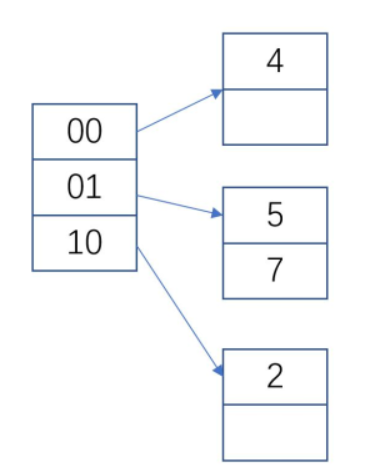
\includegraphics[width=0.95\textwidth]{1}
    \caption{蛋白质的四级结构}
    \label{fig:1.1}
\end{figure}

\section{算法简介}
\subsection{问题概述}
AlphaFold解决的问题是蛋白质折叠问题,可以抽象成如下:

输入:Alpha Fold的输入是一个氨基酸序列,每一个位置的元素代表了链上的一个氨基酸单元(一共可以有21种氨基酸单元),一个典型的输入如下:

PIAQIHILEGRSDEQKETLIREVSEAISRSLDAPLTSVRVIITEMAKGHFGIGGELASK

这个输入代表是一个包含59个氨基酸的链。

输出:在接收到这个单一序列的输入之后,AlphaFold需要使用算法,预测这一个氨基酸链条会如何折叠,所以输出的是一个拓扑结构。上面这段氨基酸输入经过AlphaFold模型运算之后输出的氨基酸拓扑结构如\cref{fig:1.2}。

\begin{figure}[H]
    \centering
    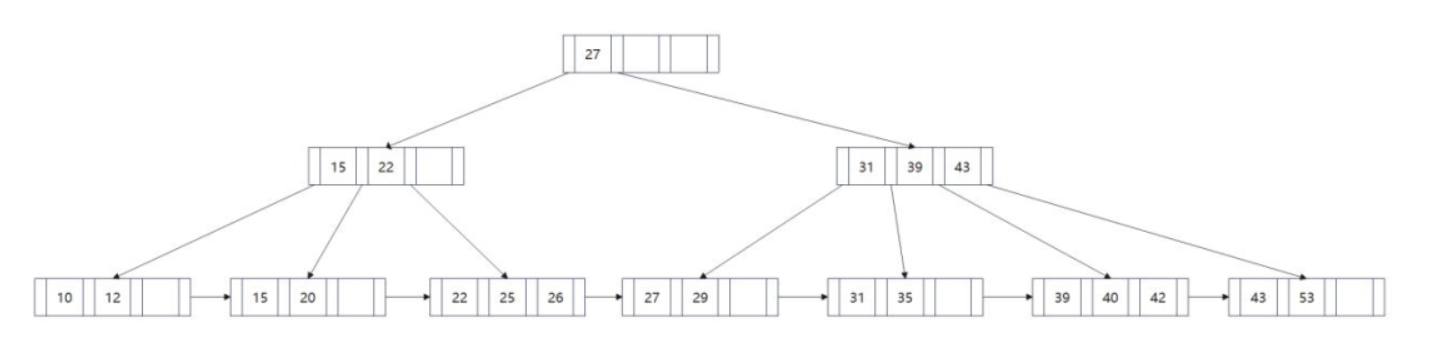
\includegraphics[width=0.95\textwidth]{2}
    \caption{氨基酸拓扑结构}
    \label{fig:1.2}
\end{figure}

当然而这个拓扑结构本身肯定不能作为输出,作为输出肯定需要是结构化的数据。准确的说,输出的数据是每一个氨基酸单元和其下一个氨基酸单元在空间中的夹角,由于是三维空间,所以说明一个方位需要2维数据,$(\varphi,\psi)$,所以AlphaFold的模型的输出就是一组数量和输入对应的夹角对。

\subsection{算法框架}
\begin{figure}[H]
    \centering
    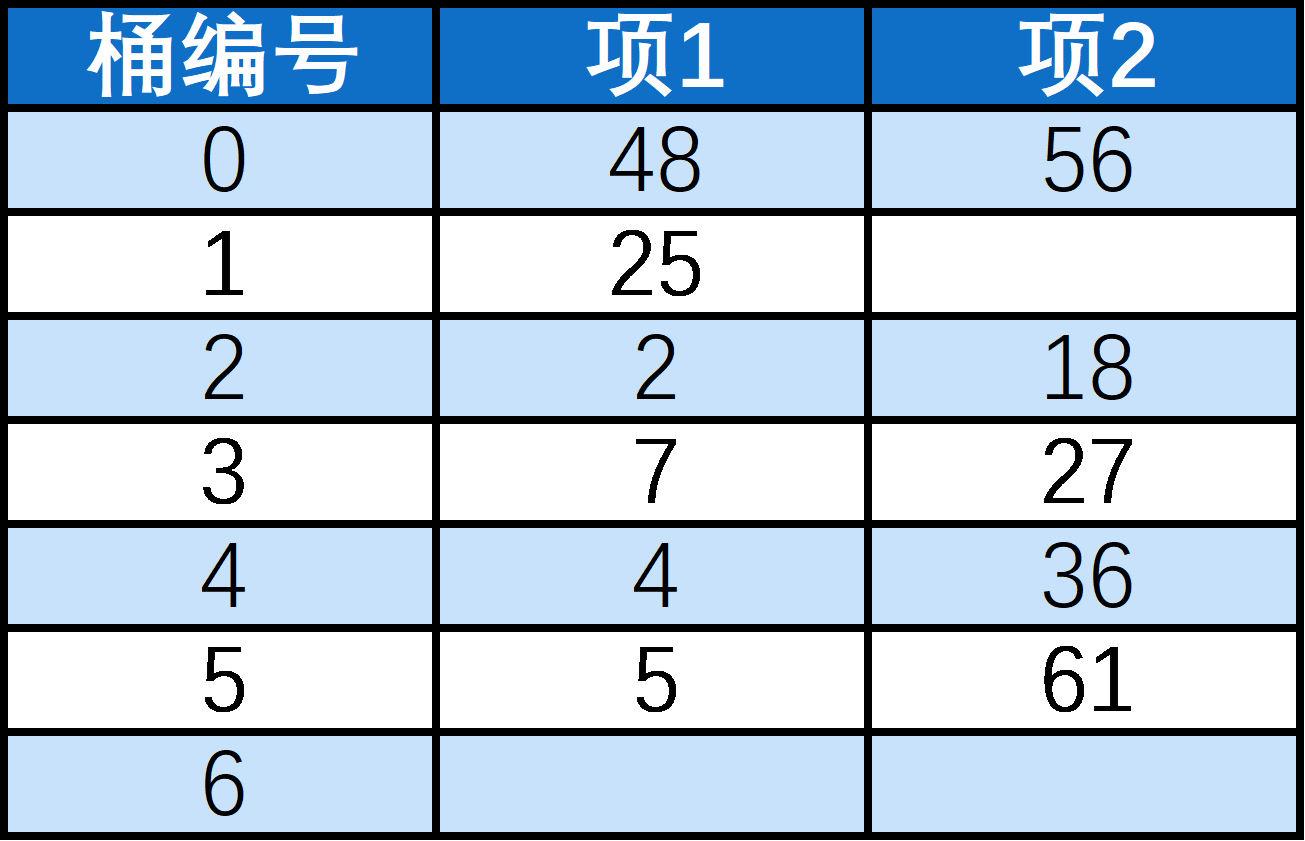
\includegraphics[width=0.95\textwidth]{3}
    \caption{AlphaFold框架}
    \label{fig:2.1}
\end{figure}

如\cref{fig:2.1},整个AlphaFlod算法可以分为以下四个部分:

\begin{enumerate}
    \item 序列和MSA特征抽取;
    \item 深度神经网络结构预测;
    \item 评估函数的构建;
    \item 结构生成。
\end{enumerate}

下面分别进行描述。

\subsubsection{特征提取}
AlphaFold的特征提取包含了序列特征和序列平方特征两大部分。

首先是序列特征,序列特征是长度和原始输入序列相同的,包括了one-hot的氨基酸种类特征(21维),HHblit特征(22维),MSA特征等等,类似的很多其他特征也被加入到序列特征中用于丰富特征表达能力。

如果输入的氨基酸序列长度为k,那么序列特征的矩阵就是一个维度为$(k,m)$的矩阵,其中$m$是序列特征的总维度。

其次就是序列平方特征,与序列特征不同,如果输入的氨基酸长度为$k$,那么序列平方特征的就会是一个维度为$(k,k,n$)的矩阵($n$为序列平方特征的数量)。这里实际上是将另一个模型即CCMpred的输出作为AlphaFlod的输入,CCMpred模型是一个用于预测氨基酸折叠后两两接触概率的模型。

AlphaFold将这个概率图和其模型参数一并加入到输入的feature中,由于这个特征是针对两两氨基酸对构造的,所以其属于序列平方特征。


\subsubsection{结构预测}

结构预测网络承担了预测蛋白质折叠后的性质的作用。这里需要注意,预测的是蛋白质的性质(包含氨基酸之间两两的距离分布,氨基酸链的夹角分布),而不是直接预测结构本身。

为了深入理解这一点,先来详细看一下结构预测模型的输入/输出。模型的输入包含了特征抽取后的序列特征和序列平方特征。假设模型的输入是一条长度为$k$的氨基酸序列,那么模型的输出包含两个部分:

\begin{enumerate}
    \item 一个$(k,k,64)$维度的输出,代表预测的两两氨基酸单元之间的距离分布,这个输出是距离的概率分布,$64$代表的是将$2-22Å$($1Å=10^{-10}m$,是一个距离单位)划分为64个桶,网络输出两两氨基酸的距离落在相应的桶里的概率
    \item 一个$(k-1,1296)$维度的输出,$1296 = 36^2$,这个输出代表每一个氨基酸和其后一个氨基酸的相对方位夹角,上文有提到,这个夹角应该用两个维度表示:$(\varphi_1,\psi_1),(\varphi_2,\psi_2),(\varphi_3,\psi_3),\dots$,但是这里AlphaFold的处理比较暴力,直接将每个360度划分成36个桶,这样一个夹角对就可以落到1296个桶中的一个,网络仍然是预测每个氨基酸对和后一个的夹角落在每个桶中的概率。
\end{enumerate}

之所以不使用预测的氨基酸链夹角作为输出,原因如下:
\begin{enumerate}
    \item 直接使用网络预测的氨基酸链夹角作为输出没有考虑其他约束,特别是氨基酸对的距离约束,而氨基酸对的距离正好神经网络比较擅长预测
    \item 氨基酸链夹角预测精度其实很差,夹角预测只能给出5度的精度(每个桶10度),而氨基酸链很长,即使一点点的角度预测偏差,都会造成累积误差,从而堆积成不可逆转的巨大偏差
    \item 即使直接使用回归来预测精确的角度,仍然会因为累积误差堆积而使得结果不可用
\end{enumerate}

\subsubsection{评估函数的构建}

这一部分的主要任务是构造一个可微函数,这个可微函数输入为一组夹角$(\varphi_1,\psi_1)$,$(\varphi_2,\psi_2)$,$(\varphi_3,\psi_3)$,$\dots$。函数输出值越小,代表这一组夹角是更好的预测结果。

假设输入的氨基酸链长度为$k$,则可以从角度输入通过简单的三角函数计算得到$(k,k)$的距离矩阵$D$。在上文中提到,AlphaFold模型已经给出预测的距离分布和角度分布。则可以得出关于距离和角度的两个公式,以及其综合之后得出的总的评价函数如式\cref{eq:2.1}。
\begin{equation}
    \begin{cases}
         & V_{distance}(X)=-\sum_{i,j,i\neq j}{\log{P(d_{ij}|S,MSA(S))}}                                         \\
         & V_{torsion}(\varphi,\psi)=-\sum_i{\log{p_{vonMiss}(\varphi_i,\psi_i)|S,MSA(S)}}                       \\
         & V_{total}=V_{distance}(G(\varphi,\psi))+V_{torsion}(\varphi,\psi)+V_{score2\_smooth}(G(\varphi,\psi))
    \end{cases}
    \label{eq:2.1}
\end{equation}

其中$score2\_smooth$项为加入的范德华项。根据上文,可以通过$(\varphi,\psi)$推导出距离矩阵$D$,这里用$G(\varphi,\psi)$代表这一过程。

\subsubsection{结构生成}

有了网络结构以及损失函数,只需使用梯度下降法求解$V_{total}(\varphi,\psi)$即可得出最优的角度值。同时为了避免梯度下降陷入局部最优解,AlphaFlod算法采用了以下方法与梯度下降法相结合来避免陷入局部最优:
\begin{itemize}
    \item 初始从结构网络的预测中采样多组$\varphi,\psi$值;
    \item 使用L-bfgs(一种梯度下降法),分别针对这几组$\varphi,\psi$值进行梯度下降优化;
    \item 维护20组最低$V_{total}(\varphi,\psi)$值的$\varphi,\psi$对;
    \item 当$\varphi,\psi$对的池子满了之后,向当前$V_{total}(\varphi,\psi)$值最低的$\varphi,\psi$对中添加噪音,然后充满整个池子,然后对每个$\varphi,\psi$对重复梯度下降过程。
\end{itemize}

结构生成模块也是AlphaFold的最后一个模块,在这个模块的算法运行完毕之后,$V_{total}(\varphi,\psi)$值最低的一组$\varphi,\psi$对被输出作为整个AlphaFold模型的预测。

\end{document}